\section{Examples}

\subsection{Pointing a telescope}
%%%%%%%---- BEGIN ----  ----%%%%%%
\begin{frame}
  \frametitle{Pointing a telescope}

  \begin{overlayarea}{\textwidth}{0.15\textheight}
    \vspace{-0.5em}
    \begin{exampleblock}{Example}
      Where do I point the telescope from the name of a target?
    \end{exampleblock}
  \end{overlayarea}

  \begin{overlayarea}{\textwidth}{0.8\textheight}
    \begin{onlyenv}<2>
      \begin{block}{Answer: CDS, IMCCE Miriade, JPL SSD, MPC, Lowell AstEph}
        \hspace{.10\hsize}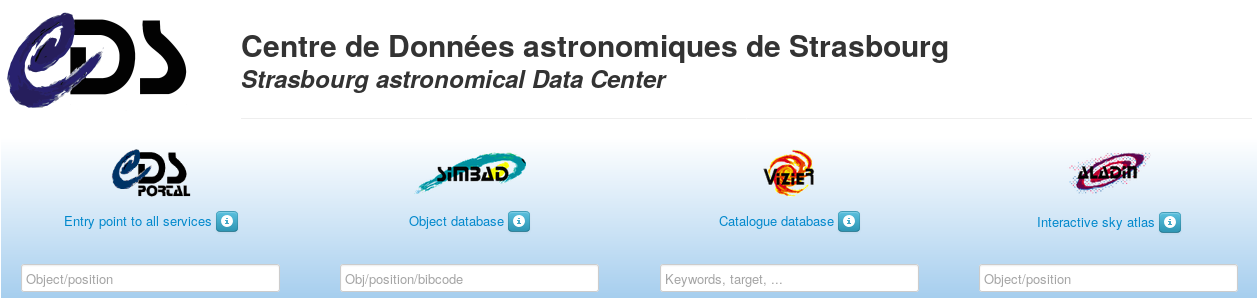
\includegraphics[width=.45\hsize]{portal-cds}\\
        \hspace{.35\hsize}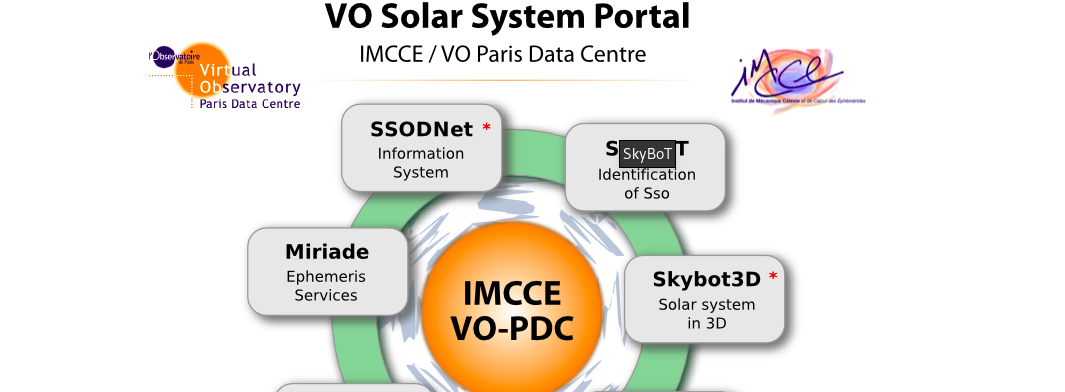
\includegraphics[width=.45\hsize]{portal-imcce}
      \end{block}
    \end{onlyenv}
  \end{overlayarea}

\end{frame}
%%%%%%%----  END  ----  ----%%%%%%


\subsection{Visibility of targets}
%%%%%%%---- BEGIN ----  ----%%%%%%
\begin{frame}
  \frametitle{Visibility of targets}

  \begin{overlayarea}{\textwidth}{0.15\textheight}
    \vspace{-0.5em}
    \begin{exampleblock}{Example}
      Can I observe asteroids Raymond, Delsanti, 7561 and 10281? And M31 and M67?
    \end{exampleblock}
  \end{overlayarea}

  \begin{overlayarea}{\textwidth}{0.8\textheight}
    \begin{onlyenv}<2>
      \begin{block}{Answer: IMCCE ViSiON, Lowell AstObs, airmass.org}
        \hspace{.25\textwidth}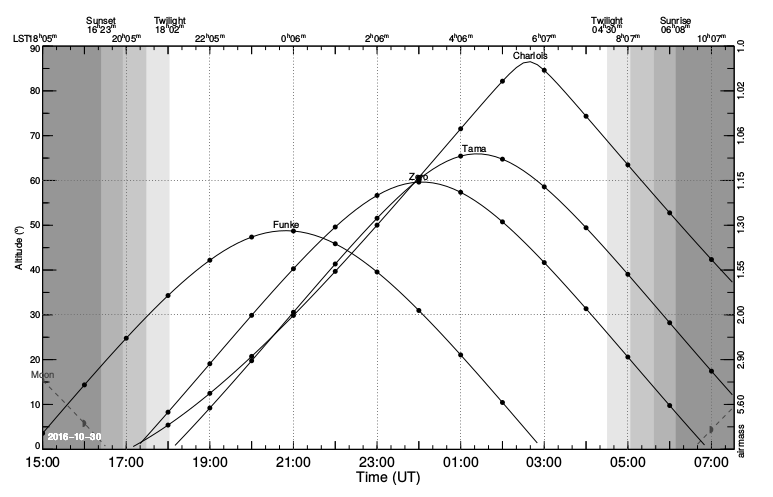
\includegraphics[width=.5\textwidth]{vision}
      \end{block}
    \end{onlyenv}
  \end{overlayarea}
% https://ssp.imcce.fr/webservices/miriade/api/vision.php?-name=a:Raymond,a:Patrickmichel,a:Libourel,a:Delsanti,u:M67,u:M31&-nbd=1&-step=1&-observer=010&-ep=2024-02-06&-from=Demo&-mime=pdf
\end{frame}
%%%%%%%----  END  ----  ----%%%%%%

\subsection{Accessing data}
%%%%%%%---- BEGIN ----  ----%%%%%%
\begin{frame}
  \frametitle{Accessing data}

  \begin{overlayarea}{\textwidth}{0.15\textheight}
    \vspace{-0.5em}
    \begin{exampleblock}{Example}
      What is the taxonomy of Vernazza? the diameter of Groussin?
    \end{exampleblock}
  \end{overlayarea}

  \begin{overlayarea}{\textwidth}{0.8\textheight}
    \begin{onlyenv}<2>
      \begin{block}{Answer: IMCCE SsODNet, JPL sbdb, OCA MP3C, Lowell AstInfo, SiMDA}
        \hspace{.05\hsize}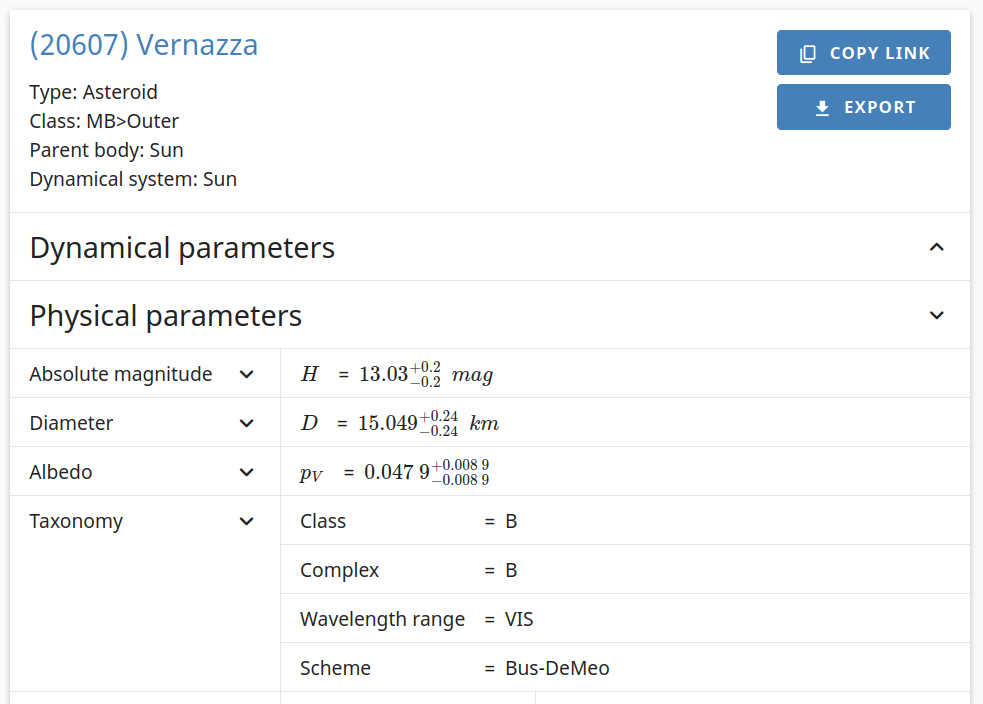
\includegraphics[width=.4\hsize]{ssodnet-vernazza}
        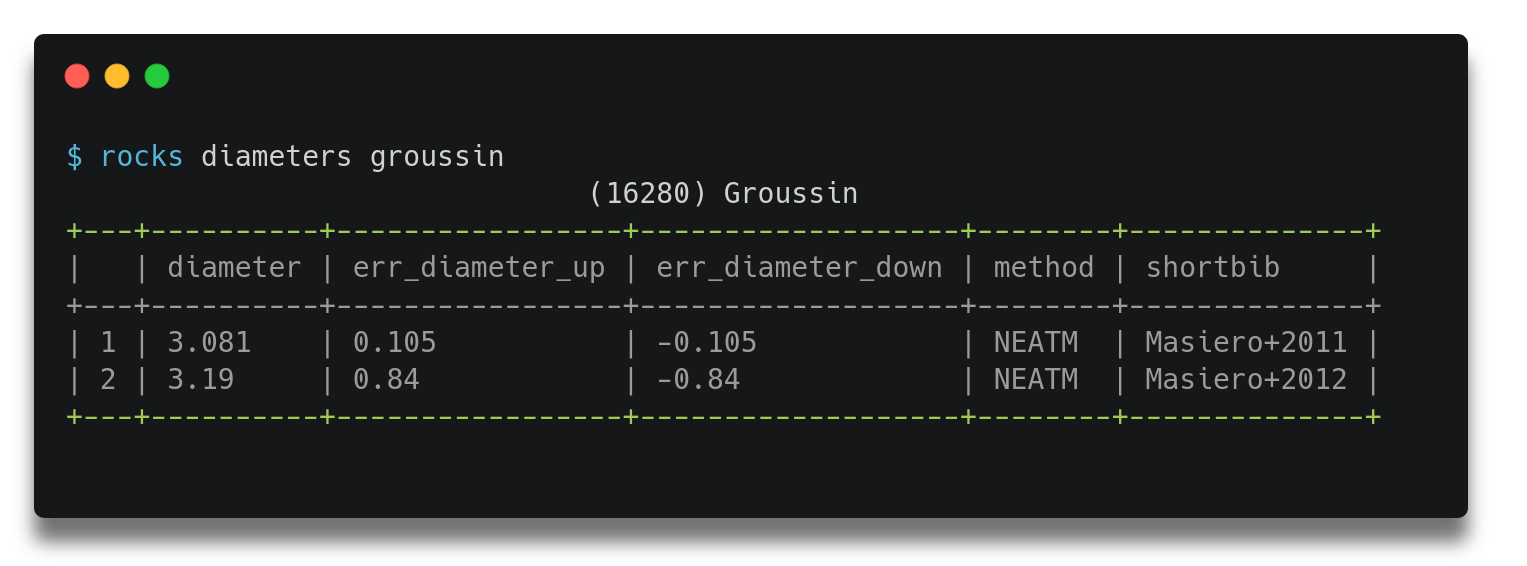
\includegraphics[width=.5\hsize]{ssodnet-groussin}
      \end{block}
    \end{onlyenv}
  \end{overlayarea}

\end{frame}
%%%%%%%----  END  ----  ----%%%%%%
